\chapter{Implementation}
\section{Plans}

Nearing the end of every sprint, the customer and group agreed upon the content of the following sprint. This list has been placed in Figure \ref{tab:sprintList}, and provided a short summary of what was accomplished in a particular time-frame. 

\section{Overall Architecture}
The product has been implement as a system of independent component applications where each component performs a well-defined task. The motivation behind the domular architecture is two-fold: Primarily, it was desirable that the underlying model for movement and fall risk be independent of the proof-of-concept application, in order to facilite development of possible future applications employing the model. Secondly, the standards of Android application development state that a Content Provider should in itself solely provide a interface to the data. This implies that the sensor model, as well as any derivation of secondary data, should be performed in components independent of the Content Provider. [ADD INFO ABOUT INDEPENDENCE SENSOR MODEL / CP AS WELL AS INDEPENDENCE CP / GUI?]

The system that has been designed according to these principles therefore consists of five components: The content provider emph{Valens Content Provider}, the proof-of-concept application emph{Valens Health Helper}, the sensor model emph{Valens Step Detector} and a service of deriving secondary data emph{Valens Content Feeder}. Each of these components fulfills a well-defined role in the total application system: The content provider provides an interface to the data model. The sensor model listens to the sensor data, and feeds the content provider with the timestamps of any detected steps. The Content Feeder listens continually to changes to the data in the content provider. When the data changes, it uses the new data to calculate secondary data, such as gait speed and variability. Finally, the proof-of-concept application demonstrates one simple way in which the data provided by the content provider can be used as a part of a health-promoting app.

\begin{figure}[p]

\setlength\fboxsep{0pt}
\setlength\fboxrule{1pt}\noindent\makebox[\textwidth]{%
 \fbox{
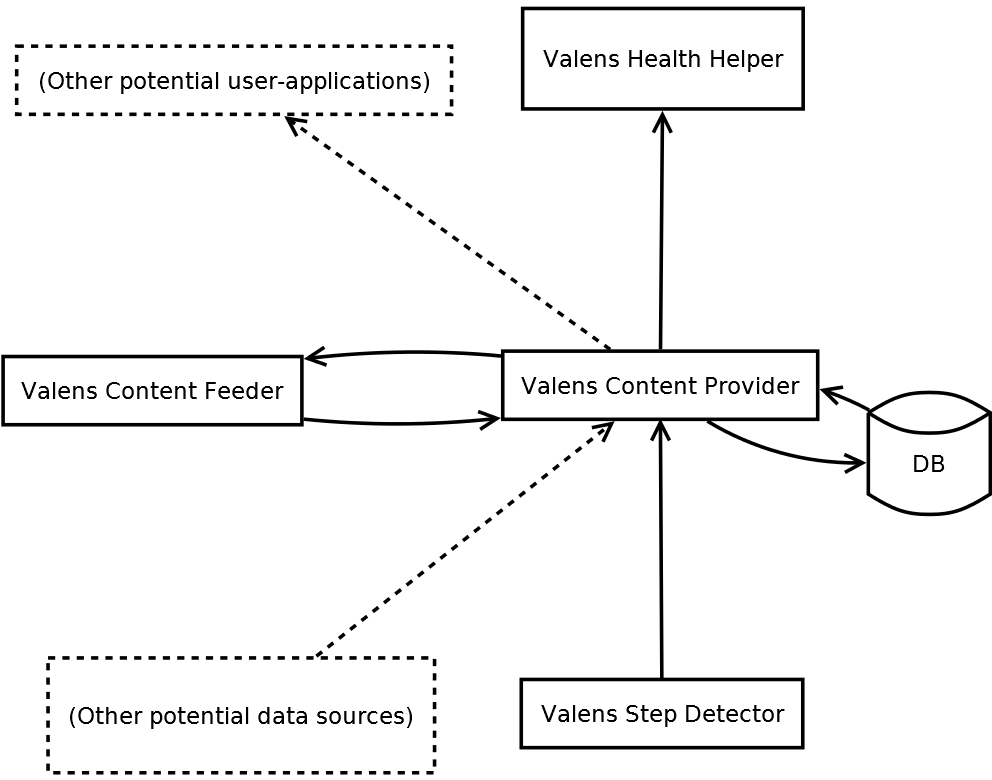
\includegraphics[width=1.45\textwidth , angle=270]{Res/OverallArchitecture}
}
}
\label{fig:Architecture}
\caption{The over-all system architecture}
\end{figure}


\section{Architecture of the App}
The application is made in a way that is common for all android applications. This means that user interface is described in xml layout files that is called in java code. Strings and resources is placed in a separate folder and file, to be accessed by the code as needed. This is to separate content and layout in the UI. The separation of layout and strings enables different localizations, so that the application can provide a user interface in different languages easily.

As is common in android applications, classes that inherit from the class Activity define a separate screen in the GUI. Because of this, a significant part of all the classes in the application are activity classes. These classes simply define the behavior of their GUI screen. The flow for the GUI can be seen in Figure \ref{fig:FlowchartGUI}
\begin{figure}
\setlength\fboxsep{0pt}
\setlength\fboxrule{1pt}\noindent\makebox[\textwidth]{
\fbox{
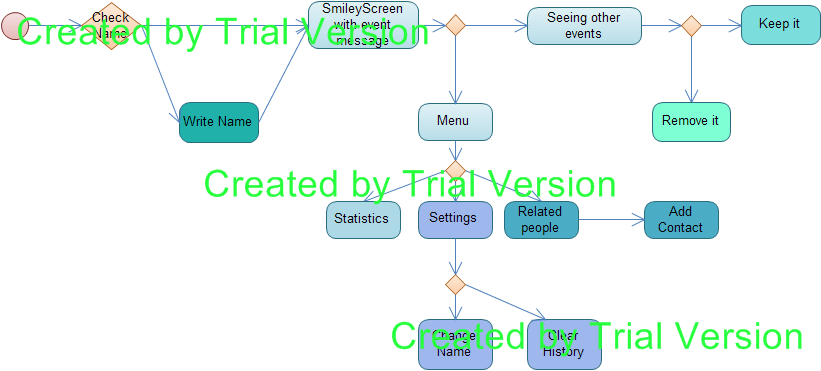
\includegraphics[width=1.2\textwidth, angle = 270]{Res/FlowChartGUI.png}
}
}
\caption{Flow chart describing the Graphical User Interface}
\label{fig:FlowchartGUI}
\end{figure}

Classes that are not activities can be roughly divided into 4 types: Data structure classes, auxiliary classes, connectivity classes, widget classes. Data structure classes simply define a useful data structure in the program. The data structure classes in the app are Event, ContactPerson and RiskStatus. Auxiliary classes help the activities perform their tasks. Most common among these are the adapters that define how elements should be shown in a list view. Connectivity classes are responsible for communicating with the database and content providers. There are two connectivity classes: DatabaseHelper, which does all the work, and DatabaseContract, which specifies the table and column names in the database. While a DatabaseContract might seem redundant, it is common android application practice to use one. Finally, there are the widget classes. WidgetProvider creates the widget and gives it a GUI. WidgetUpdateService is started by the WidgetProvider and takes care of updating the widget when changes happen in the content provider.

\section{Architecture of the Content Provider}
In android, Content Providers provide an interface to structured data of some sort. Access to for instance the list of contacts in the phone, or the phone's calendar is managed through standard content providers. Content Providers provide methods for inserting, updating and deleting relevant data. A major part of the assignment was to implement a Content Provider that gives developers access to structured movement data.

The Content Provider component is conceptually very simple, and consists of four classes:
\begin{description}
\item[CPValensDB]
a subclass of SQLiteOpenHelper, the standard android class for handling database communication. Specifies the procedure for creating the database, as well as upgrading and downgrading the database version. In the current implementation, upgrading and downgrading the database version clears all the data and tables, and creates the database according the details specified in the new database version. In the current version, creating the database consists of creating the tables given in the data model, without feeding any data into the database.
\item[DBSchema]
defines the database model and provides string values for the names of the tables and fields. Employing a database schema to demonstrate the structure of the database is standard in android applications.
\item[ValensDataProvider]
a subclass of ContentProvider, which is the standard android class for implementing content providers. This is the core of the content provider, and describes how queries to the content provider are handled.
\item[Main]
provdides the content provider with a basic GUI.
\end{description}


\section{Class description and diagram}

The class structure of the Applications changed regularly, and the most recent description is in Figure \ref{fig:ClassDiagram}. Older diagrams and descriptions was placed in the appendix. 
\begin{figure}[p]
\label{fig:ClassDiagram}

\setlength\fboxsep{0pt}
\setlength\fboxrule{1pt}
\fbox{
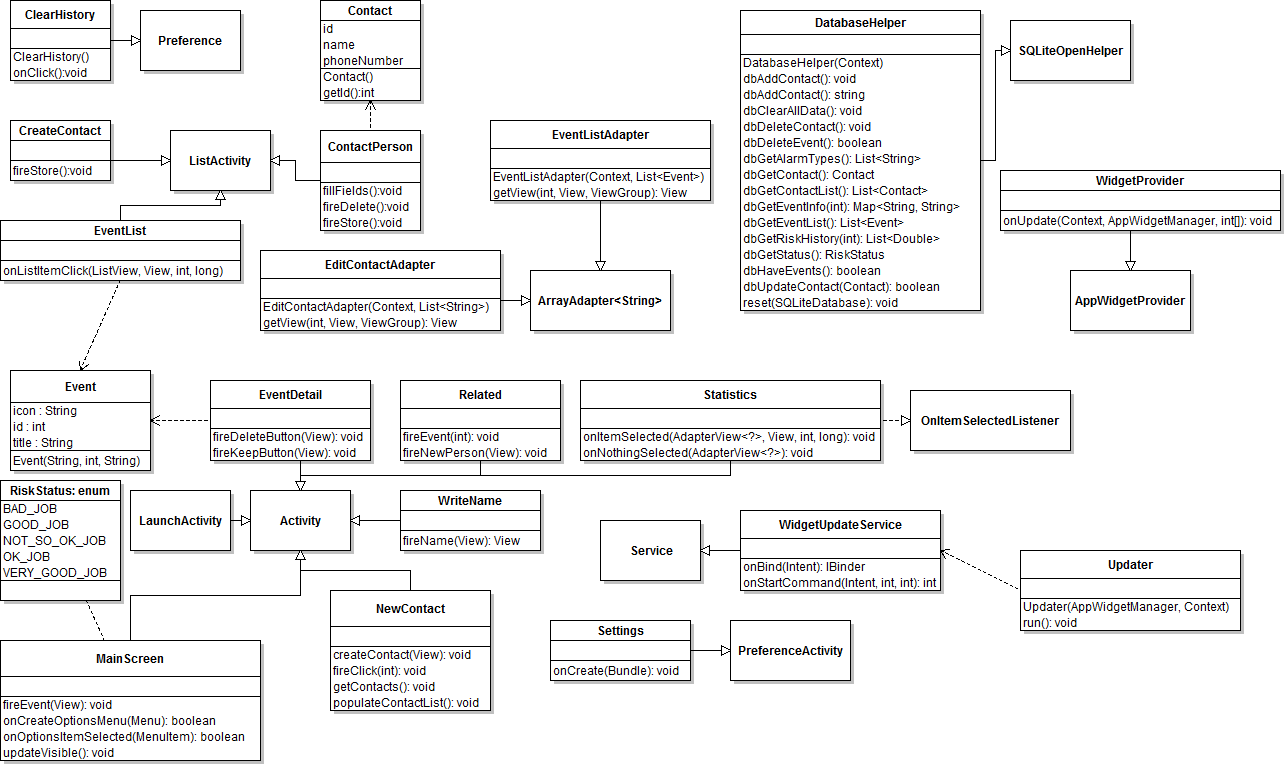
\includegraphics[width=1.2\textwidth, angle = 270]{Res/ClassDiagram}
}
\caption{A class diagram of the current application}
\end{figure}

\section{Architecture of the Valens Step Detector}

Despite being a relatively simple application in terms of lines of code and GUI screens, the architecture of Valens Step Detector has a certain complexity.
